\documentclass[11pt]{article}
\usepackage[a4paper,margin=1.5cm]{geometry}
\usepackage[T1]{fontenc}
\usepackage[scaled]{helvet}
\renewcommand{\familydefault}{\sfdefault}
\usepackage{tikz}
\usetikzlibrary{positioning,arrows.meta,calc}
\usepackage{xcolor}

\definecolor{ebOrange}{HTML}{FF7026}
\definecolor{depotBlue}{HTML}{2563EB}
\definecolor{groupOrange}{HTML}{EA580C}
\definecolor{sroGreen}{HTML}{059669}
\definecolor{ink}{HTML}{1F2937}
\definecolor{soft}{HTML}{6B7280}
\definecolor{paper}{HTML}{F9FAFB}

\newcommand{\arr}{\textcolor{soft}{$\rightarrow$}}
\pagestyle{empty}

\begin{document}
\begin{center}
{\Large\bfseries Echo Barrier — Intercompany PO Flow}\\[3pt]
{\color{soft}\small Raise in the Hub \;·\; approve \;·\; authorise across Depot $\rightarrow$ Group $\rightarrow$ SRO Xero \;·\; trace by the Group PO\#}
\end{center}
\vspace{5mm}

\begin{center}
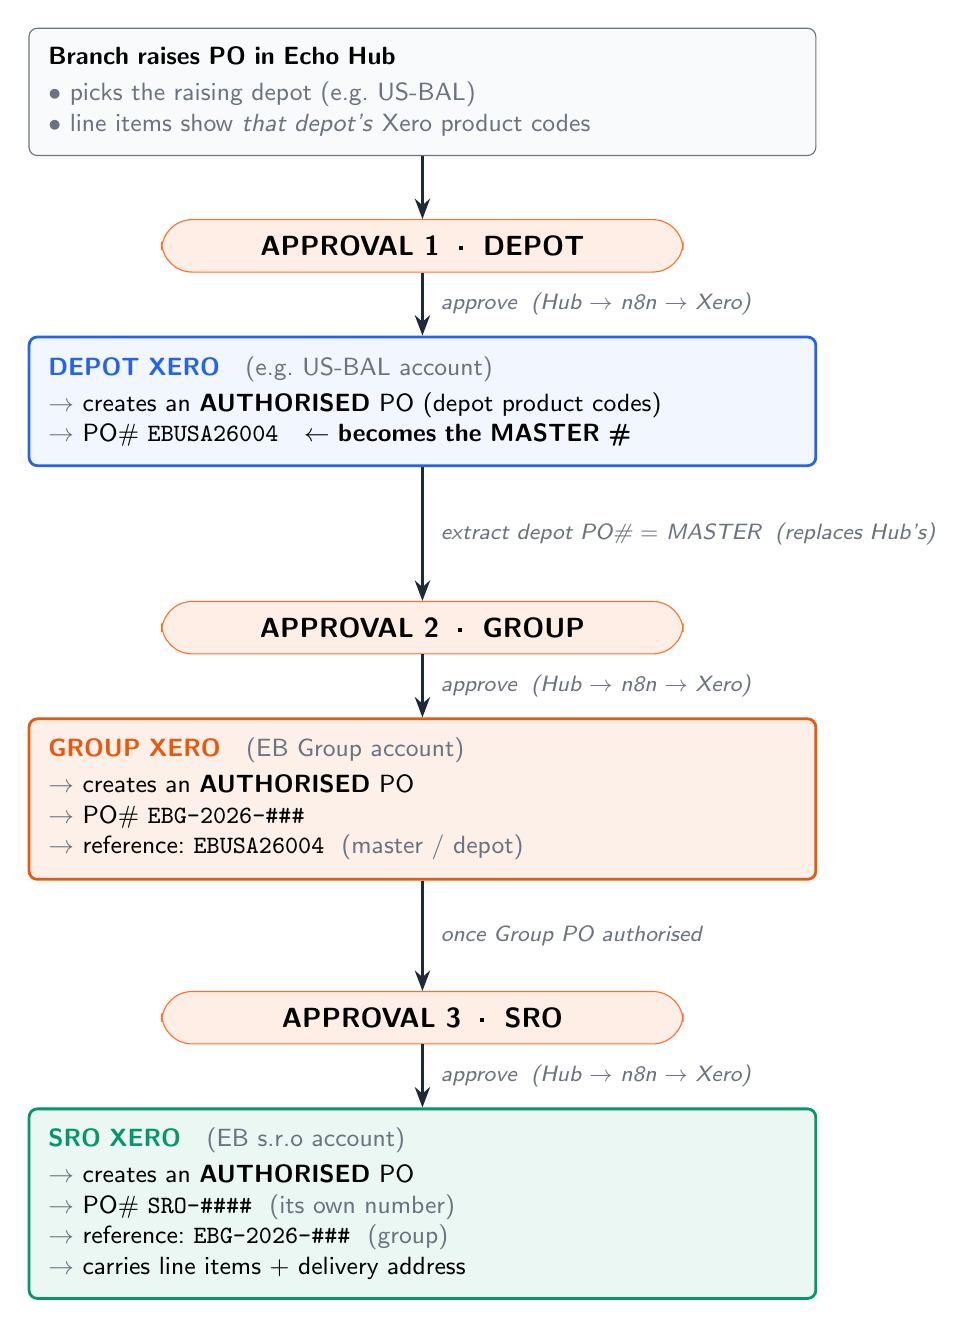
\begin{tikzpicture}[
  font=\small,
  >={Stealth[length=2.6mm]},
  base/.style={rounded corners=3pt, draw, align=left, inner sep=7pt, text width=95mm},
  raise/.style={base, fill=paper, draw=soft},
  gate/.style={rounded corners=11pt, draw=ebOrange, fill=ebOrange!12, align=center,
               inner sep=6pt, text width=62mm, font=\bfseries},
  xero/.style={base, line width=1pt},
  flow/.style={->, line width=0.9pt, color=ink},
  lbl/.style={midway, right, font=\footnotesize\itshape, color=soft, xshift=1mm}
]

\node[raise] (raise) {%
  \textbf{Branch raises PO in Echo Hub}\\[2pt]
  \textcolor{soft}{$\bullet$ picks the raising depot (e.g.\ US-BAL)}\\
  \textcolor{soft}{$\bullet$ line items show \emph{that depot's} Xero product codes}};

\node[gate, below=8mm of raise] (g1) {APPROVAL 1 \;·\; DEPOT};

\node[xero, draw=depotBlue, fill=depotBlue!6, below=8mm of g1] (depot) {%
  \textbf{\textcolor{depotBlue}{DEPOT XERO}}\quad\textcolor{soft}{(e.g.\ US-BAL account)}\\[2pt]
  \arr\ creates an \textbf{AUTHORISED} PO (depot product codes)\\
  \arr\ PO\#\ \texttt{EBUSA26004}\quad\textbf{$\leftarrow$ becomes the MASTER \#}};

\node[gate, below=17mm of depot] (g2) {APPROVAL 2 \;·\; GROUP};

\node[xero, draw=groupOrange, fill=groupOrange!9, below=8mm of g2] (group) {%
  \textbf{\textcolor{groupOrange}{GROUP XERO}}\quad\textcolor{soft}{(EB Group account)}\\[2pt]
  \arr\ creates an \textbf{AUTHORISED} PO\\
  \arr\ PO\#\ \texttt{EBG-2026-\#\#\#}\\
  \arr\ reference:\ \texttt{EBUSA26004}\ \ \textcolor{soft}{(master / depot)}};

\node[gate, below=14mm of group] (g3) {APPROVAL 3 \;·\; SRO};

\node[xero, draw=sroGreen, fill=sroGreen!8, below=8mm of g3] (sro) {%
  \textbf{\textcolor{sroGreen}{SRO XERO}}\quad\textcolor{soft}{(EB s.r.o account)}\\[2pt]
  \arr\ creates an \textbf{AUTHORISED} PO\\
  \arr\ PO\#\ \texttt{SRO-\#\#\#\#}\ \ \textcolor{soft}{(its own number)}\\
  \arr\ reference:\ \texttt{EBG-2026-\#\#\#}\ \ \textcolor{soft}{(group)}\\
  \arr\ carries line items + delivery address};

\draw[flow] (raise) -- (g1);
\draw[flow] (g1) -- (depot) node[lbl]{approve \;(Hub $\rightarrow$ n8n $\rightarrow$ Xero)};
\draw[flow] (depot) -- (g2) node[lbl]{extract depot PO\# $=$ MASTER \;(replaces Hub's)};
\draw[flow] (g2) -- (group) node[lbl]{approve \;(Hub $\rightarrow$ n8n $\rightarrow$ Xero)};
\draw[flow] (group) -- (g3) node[lbl]{once Group PO authorised};
\draw[flow] (g3) -- (sro) node[lbl]{approve \;(Hub $\rightarrow$ n8n $\rightarrow$ Xero)};

\end{tikzpicture}
\end{center}

\vspace{6mm}
\begin{center}
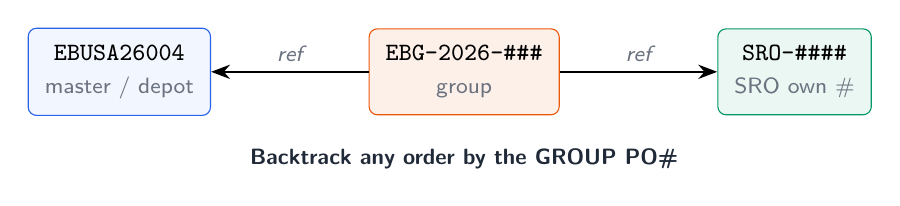
\begin{tikzpicture}[font=\small, >={Stealth[length=2.4mm]}]
\node[draw=depotBlue, rounded corners=3pt, fill=depotBlue!6, inner sep=6pt, align=center] (m)
  {\texttt{EBUSA26004}\\[1pt]\footnotesize\color{soft}master / depot};
\node[draw=groupOrange, rounded corners=3pt, fill=groupOrange!9, inner sep=6pt, align=center, right=20mm of m] (g)
  {\texttt{EBG-2026-\#\#\#}\\[1pt]\footnotesize\color{soft}group};
\node[draw=sroGreen, rounded corners=3pt, fill=sroGreen!8, inner sep=6pt, align=center, right=20mm of g] (s)
  {\texttt{SRO-\#\#\#\#}\\[1pt]\footnotesize\color{soft}SRO own \#};
\draw[<-, line width=0.9pt] (m) -- node[above, font=\footnotesize\itshape, color=soft]{ref} (g);
\draw[->, line width=0.9pt] (g) -- node[above, font=\footnotesize\itshape, color=soft]{ref} (s);
\node[below=3mm of g, font=\footnotesize\bfseries, color=ink] {Backtrack any order by the GROUP PO\#};
\end{tikzpicture}
\end{center}

\end{document}
